\documentclass{article}
\usepackage[utf8]{inputenc}
\usepackage{ graphicx }
\usepackage{ geometry}
\geometry{legalpaper, margin=1.3in}
\usepackage{ bbm }
\usepackage{ braket }
\usepackage{ mathrsfs }

\usepackage{ mathrsfs }
\usepackage{ mathtools }
\usepackage{ amsfonts }
\usepackage{ caption }
\usepackage{ tikz }
\usepackage[hidelinks]{ hyperref }

\newcommand\eqdef{\stackrel{\mathclap{\tiny\mbox{def}}}{=}}

\title{qk4cs}
\author{Hugo Thomas}
\date{2021/2022}

\begin{document}

\section*{Wave equation}
\begin{equation}
    \label{wave-equation}
    \frac{1}{c^2}\cdot\frac{\partial^2 f}{\partial t^2} - \frac{\partial^2 f}{\partial x^2} = 0
\end{equation}

The general form of the solution is $f(x, t)=g(x-ct)+h(x+ct)$
\section*{Progressive plane wave equation}
\begin{equation}
f(x, t) = A \cos{(\kappa x - \omega t)}
        = A \text{ Re}{(e^{i(\kappa x - \omega t)})}
\end{equation}

\begin{figure}[h]
\centering
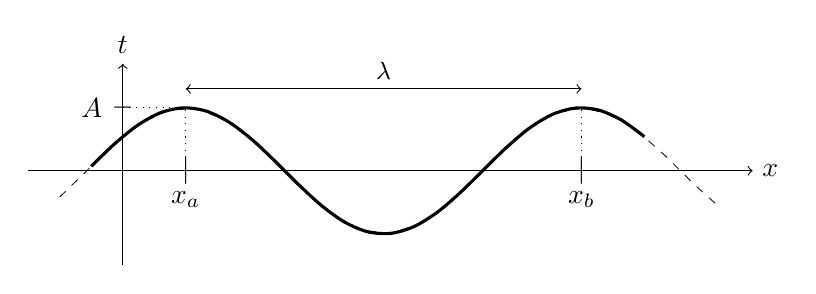
\begin{tikzpicture}[scale=0.8]
  % Axis
  \draw[->] (-1.5, 0) -- (10, 0) node[right] {$x$};
  \draw[->] (0, -1.5) -- (0, 1.7) node[above] {$t$};

  % Plot the parametrized function
  \draw[line width=0.4mm, domain=-0.5:2*(pi+1), smooth, variable=\x, black] plot(\x,{cos((\x-1) r)});

  % Plot the dashed line
  \draw[ line width=0.1mm, domain=-1:9.5, dashed, variable=\x, black] plot(\x,{cos((\x-1) r)});

  % Spot xa
  \draw[dotted] (1,0) -- (1,1);
  \draw[very thin,black] (1,0) node{$|$} node[below=4pt]{$x_a$};

  % Spot xb
  \draw[dotted] (2*pi+1,0) -- (2*pi+1,1);
  \draw[very thin,black] (2*pi+1,0) node{$|$} node[below=4pt]{$x_b$};

  % Spot A
  \draw[dotted] (0,1) -- (1,1);
  \draw[very thin,black] (0,1) node{$-$} node[left=4pt]{$A$};

  % Lambda arrow
  \draw[<->] (1,1.3) -- node[above]{\small $\lambda$} (2*pi+1,1.3);
\end{tikzpicture}
\caption{Wave : spacial representation}
\label{wave-space}
\end{figure}

\begin{figure}[h]
\centering
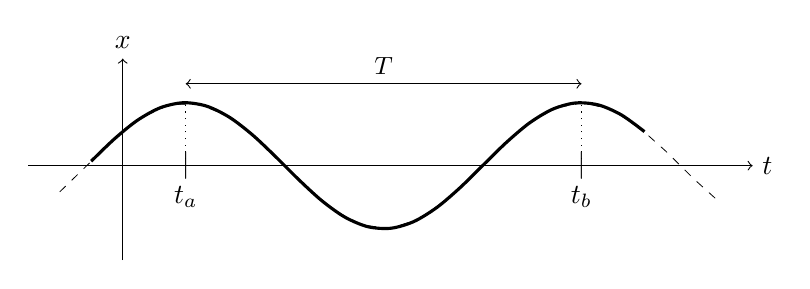
\begin{tikzpicture}[scale=0.8]
  % Axis
  \draw[->] (-1.5, 0) -- (10, 0) node[right] {$t$};
  \draw[->] (0, -1.5) -- (0, 1.7) node[above] {$x$};

  % Plot the parametrized function
  \draw[line width=0.4mm, domain=-0.5:2*(pi+1), smooth, variable=\x, black] plot(\x,{cos((\x-1) r)});

  % Plot the dashed line
  \draw[ line width=0.1mm, domain=-1:9.5, dashed, variable=\x, black] plot(\x,{cos((\x-1) r)});

  % Spot xa
  \draw[dotted] (1,0) -- (1,1);
  \draw[very thin,black] (1,0) node{$|$} node[below=4pt]{$t_a$};

  % Spot xb
  \draw[dotted] (2*pi+1,0) -- (2*pi+1,1);
  \draw[very thin,black] (2*pi+1,0) node{$|$} node[below=4pt]{$t_b$};

  % Lambda arrow
  \draw[<->] (1,1.3) -- node[above]{\small $T$} (2*pi+1,1.3);
\end{tikzpicture}
\caption{Wave : time representation}
\label{wave-time}
\end{figure}

\section*{Dispersion relation}
\hyperref[sec:wave-length-proof]{Proof p.} \pageref{sec:dispersion-relation-proof}

By plotting (2) in exponential form into (1), with found that $f$ if a wave if and only if:
\begin{equation}
    \label{dispersion}
    \kappa ^2 = \frac{\omega ^2}{c^2}
\end{equation}


\section*{Wave length relation}
\hyperref[sec:wave-length-proof]{Proof p.} \pageref{sec:wave-length-proof}
\begin{equation}
\label{wavelength}
    \lambda=\frac{2\pi}{\kappa}
\end{equation}
Where $\kappa$ is the wave number.

\section*{Period relation}
\hyperref[sec:wave-length-proof]{Proof p.} \pageref{sec:period-proof}
\begin{equation}
\label{period}
    T\eqdef\frac{1}{\nu} = \frac{\lambda}{c}
\end{equation}



\newpage
\section*{Proofs}

\subsection*{Dispersion relation (\ref{dispersion})}
\label{sec:dispersion-relation-proof}
Referring to Fig. \ref{wave-time}.

The wave is given by the equation $f(x,t) = A \text{ Re}{(e^{i(\kappa x - \omega t)})} $.

\bgroup
\def\arraystretch{2.5}
\begin{center}
\begin{tabular}{cc}
 $\dfrac{\partial f}{\partial t} = A(-i\omega)e^{i(\kappa x - \omega t)}$
 & $\dfrac{\partial^2 f}{\partial t^2} = -A\omega^2e^{i(\kappa x - \omega t)}$ \\
 $\dfrac{\partial f}{\partial x} = A(i\kappa)e^{i(\kappa x - \omega t)}$
 & $\dfrac{\partial f}{\partial x^2} = -A\kappa^2e^{i(\kappa x - \omega t)}$\\
\end{tabular}
\end{center}
\egroup

Using the equation (\ref{wave-equation}), we obtain the relation
$$
-\frac{\omega^2}{c^2} + \kappa^2 = 0
$$

Hence, $f$ is a wave if and only if
$$
\kappa ^2 = \frac{\omega ^2}{c^2}
$$


\subsection*{Wave length (\ref{wavelength})}
\label{sec:wave-length-proof}
Referring to Fig. \ref{wave-space}.
$$
\begin{aligned}
    f(x_b, t) & = f(x_a, t) \\
    A \cos{(\kappa x_b - \omega t)} & = A \cos{(\kappa x_a - \omega t)} \\
    \kappa x_b - \omega t & = \kappa x_a - \omega t + 2\pi \\
    \kappa (x_b - x_a) & = 2\pi \\
    x_b - x_a & = \frac{2\pi}{\kappa}\\
    \lambda & = \frac{2\pi}{\kappa}
\end{aligned}
$$

\subsection*{Period (\ref{period})}
\label{sec:period-proof}
\begin{figure}[h]
\centering
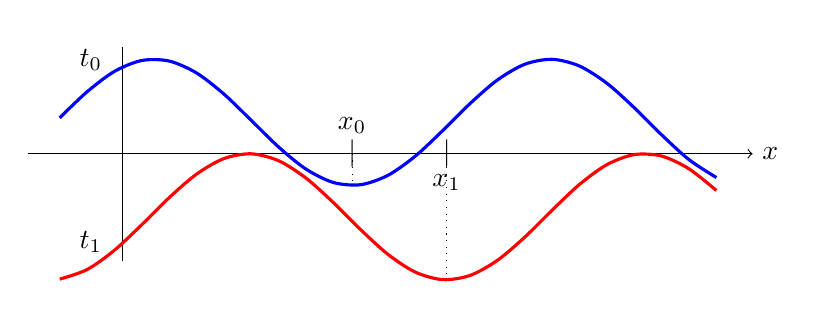
\begin{tikzpicture}[scale=0.8]
  % Axis
  \draw[->] (-1.5, 0) -- (10, 0) node[right] {$x$};
  \draw[-] (0, -1.7) -- (0, 1.7) node[above] {};

  % Plot the parametrized function
  \draw[line width=0.4mm, domain=-1:3*(pi), smooth, variable=\x, blue] plot(\x,{cos((\x-0.5) r)+0.5});

  \draw[ line width=0.4mm, domain=-1:3*(pi), smooth, variable=\x, red] plot(\x,{cos((\x-2) r)-1});

  % Spot x0
  \draw[dotted] (pi+0.5,0) -- (pi+0.5,-0.5);
  \draw[very thin,black] (pi+0.5,0) node{$|$} node[above=4pt]{$x_0$};

  \draw[very thin,black] (0,1) node{} node[above left=4pt]{$t_0$};

  \draw[very thin,black] (0,-0.9) node{} node[below left=4pt]{$t_1$};

  % Spot x1
  \draw[dotted] (pi+2,0) -- (pi+2,-2);
  \draw[very thin,black] (pi+2,0) node{$|$} node[below=4pt]{$x_1$};

\end{tikzpicture}
\caption{Delayed waves}
\label{wave-period-proof}
\end{figure}

Considering Fig. \ref{wave-period-proof}, the red wave is delayed from the blue one by a time $t_1-t_0$. And we have the following equality.

$$
\begin{aligned}
    e^{i(\kappa x_0 - \omega t_0)} & = e^{i(\kappa x_1 - \omega t_1)} \\
    \kappa x_0 - \omega t_0 & = \kappa x_1 - \omega t_1 \\
    \omega(t_1-t_0) & = \kappa(x_1-x_0) \\
    x_1-x_0 & = \frac{\omega}{\kappa}(t_0-t_1)
\end{aligned}
$$

And $c = \frac{\omega}{\kappa}$, $\lambda = x_1-x_0$, $T = t_0-t_1$. Hence $T = \frac{\lambda}{c}$.

\end{document}